\hypertarget{trossen-geekbots}{%
\section{Trossen GeekBots}\label{trossen-geekbots}}

In the course of this text we have seen several different robot
topologies but have focused a significant amount of time on the simple
differential-drive robot. To accompany the text a basic
differential-drive robot has been developed and deployed. The donor
chassis for this specific design is the (now defunct) RobotGeeks
GeekBot, from which we will appropriate a name. The GeekBot as
constructed for use with this text has been developed with cost in mind:
total parts cost comes in at just below \$300. A 3D printer was used to
print one mount for the SBC as well as a mount for the infrared sensor.
All files will be made available online for the aspiring roboticist.

The purpose of the SDSMT GeekBot is to teach the basics of robot control
using ROS on physical hardware. To accomplish this task the familiar
RobotGeeks GeekBot platform was used as a mobile base and extra hardware
added as needed.

\hypertarget{hardware}{%
\subsection{Hardware:}\label{hardware}}

\hypertarget{locomotion}{%
\subsubsection{Locomotion}\label{locomotion}}

The GeekBot comes stock with two drive wheels, powered by 6v
continuous-rotation hobby servos. Two caster balls keep the bot vertical
with a bit of wobble. These motors are not encoded, meaning they only
have relative speed adjustment. The actual angular velocity of the
wheels is unknown at any point other than stopped. Important: these
motors are run directly off the unregulated input power supply. These
motors will cook if supplied with more than \textasciitilde8.5v.

\hypertarget{electrical}{%
\subsubsection{Electrical}\label{electrical}}

The GeekBot is supplied by an 8.4v 2.2Ah LiPo battery. This is 8.4v is
passed straight to the drive motors, the onboard Arduino, and a 5v
regulator for supplying the Odroid XU4. The harness switches power to
the system, and a disconnect is located on the back to decouple battery
power and allow the use of another \textless9v supply for testing.

\hypertarget{sensors}{%
\subsubsection{Sensors}\label{sensors}}

The GeekBot has two sensors: a front-mounted webcam and a servo-actuated
IR distance sensor. The IR sensor is mounted under the front of the
robot and centered forward; the full range of motion encompasses 0-180
degrees. This sensor returns a non-linear analog voltage corresponding
to perceived distance that is passed to the onboard Arduino and
processed. The mounted webcam is is both powered by and communicates
over one of the Odroid's USB ports. This particular webcam is manual
focus and captures at 640x480px, 30fps.

\hypertarget{compute-and-control}{%
\subsubsection{Compute and control}\label{compute-and-control}}

The GeekBot follows a standard distributed-control topology: a
high-level controller issues commands to low-level controllers which
handle command implementation for specific subsystems. In this case, the
high-level controller is an Odroid XU4 running a minimal version of
Ubuntu 16.04 LTS. All hardware interfacing tasks (driving servos,
reading voltages, turning lights on) are controlled by the Arduino,
taking commands from the Odroid via UART. Below you can see a quick
graphic showing these interconnects.

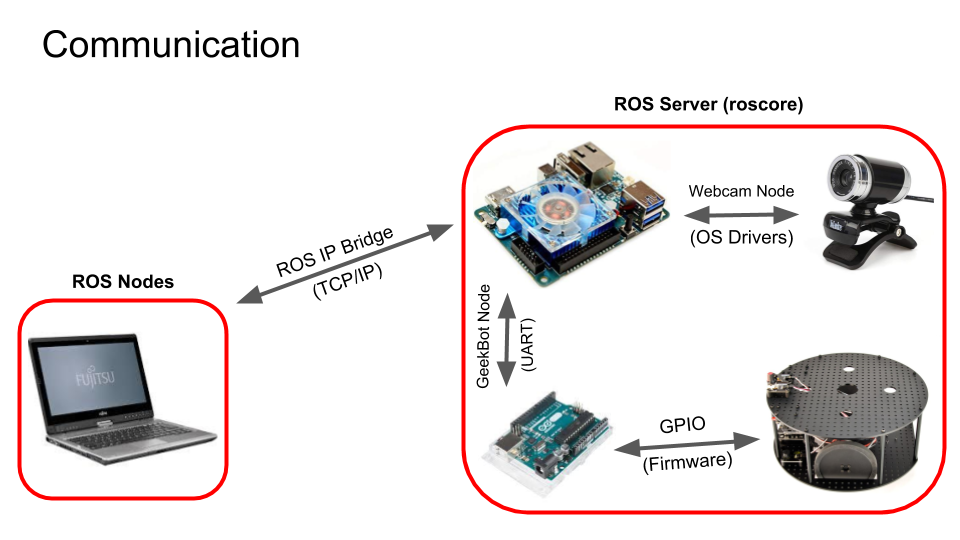
\includegraphics[width=0.75\textwidth,height=\textheight]{figures/geekbot/graphics/comm_graphic.png}

You will note that there are many, many places for communication
failures (cut wires, unplugged cables, etc.) in this setup.
Unfortunately this is one of the downfalls of real robotics;
communications will eventually fail and you will have to have systems in
place to guarantee correct data transfer or robot sutdown. For now, and
at our own risk, we'll assume that there will be no communication
interruptions in the GeekBot system.

\hypertarget{software}{%
\subsection{Software:}\label{software}}

\hypertarget{ros-kinetic}{%
\subsubsection{ROS Kinetic}\label{ros-kinetic}}

Despite the rest of the text using ROS2 Ardent, the GeekBot runs ROS1
Kinetic. The reasoning behind this decision pertains mostly to the lack
of documentation, compressed image transport, networking tools, and
debugging tools in ROS2 as of publishing time. The concepts presented in
this text for ROS2 are directly transferable to ROS Kinetic. Nodes run
independently of each other and communicate via passing messages over
topics, exactly like ROS2. ROS1, however, does have a supervisory piece
of software called \texttt{roscore} which handles node connections and
message direction.

\hypertarget{software-architecture}{%
\subsubsection{Software architecture}\label{software-architecture}}

On boot the GeekBot ROS subsystem starts up three things: roscore, for
handling all communications; a node to handle webcam things (webcam),
and another node to handle communication with the Arduino
(geekbot\_node). Both exist under the \texttt{/geekbot} namespace. Using
ROS' node/topic mapping tool \texttt{rqt\_graph} we can see the
GeekBot's nodes, topics, and the namespace under which all of these
exist.

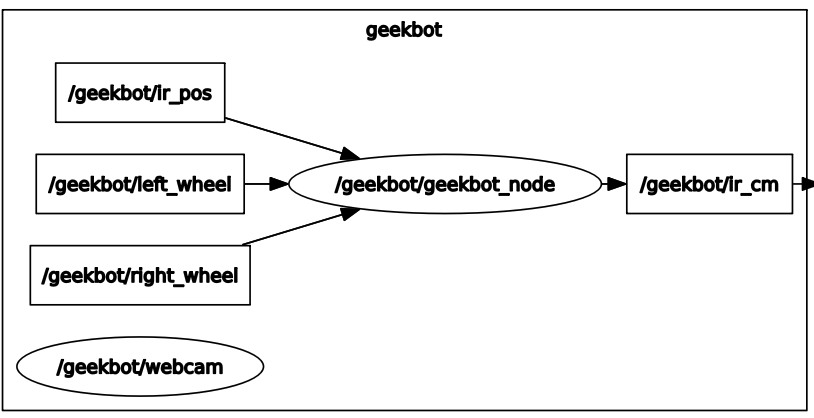
\includegraphics[width=0.75\textwidth,height=\textheight]{figures/geekbot/graphics/geekbot_nodes.png}

Bringup on boot is handled by a service through \texttt{systemd} that
points to a script contained in the \texttt{geekbot\_pkg} package which
resides within the \texttt{geekbot\_ws} directory in the \texttt{/root}
directory of the Odroid's filesystem. Handling bringup through
\texttt{systemd} allows for synchronization with the networking stack as
well as an easy start-stop-restart interface so the GeekBot's ROS system
can be restarted with the robot powered up and online. Linking to a
\texttt{systemd} service in a repository-held package gives the option
for updates to bringup handling without requiring extensive filesystem
rework. Using a \texttt{systemd} service to start ROS systems on boot is
much less common than simply pushing a start script to \texttt{init.d},
\texttt{rc.local}, or \texttt{cron} and is certainly more work to set
up. However, using \texttt{systemd} allows for much simpler
logging/debugging, runtime adjustments to the underlying ROS subsystem,
and (most importantly) hardware-specific startup criterion using
\texttt{udev} rules to adjust targets. We won't get into implementing
such things here.

\hypertarget{published-topics}{%
\subsubsection{Published topics}\label{published-topics}}

After being powered on and being assigned an IP address in the 10.42.0.X
range the GeekBot will publish/subscripe to several topics. The topics
we care about are as follows:

\begin{quote}
\begin{description}
\item[\textbf{/geekbot/ir\_cm}]
\begin{itemize}
\tightlist
\item
  Publishes: Int32
\item
  Distance to nearest object in centimeters as seen by the IR sensor
\end{itemize}
\item[\textbf{/geekbot/ir\_pos}]
\begin{itemize}
\tightlist
\item
  Subscribes: Int32
\item
  Angle (0-180) at which to set the IR sensor's servo
\end{itemize}
\item[\textbf{/geekbot/left\_wheel}]
\begin{itemize}
\tightlist
\item
  Subscribes: Int32
\item
  Relative speed (-100-100) at which to set the left wheel. Negative for
  reverse
\end{itemize}
\item[\textbf{/geekbot/right\_wheel}]
\begin{itemize}
\tightlist
\item
  Subscribes: Int32
\item
  Relative speed (-100-100) at which to set the right wheel. Negative
  for reverse
\end{itemize}
\item[\textbf{/geekbot/webcam/image\_raw}]
\begin{itemize}
\tightlist
\item
  Publishes: Image
\item
  Raw image from the camera, with zero compression of any kind. Very
  large message
\end{itemize}
\item[\textbf{/geekbot/webcam/image\_raw/compressed}]
\begin{itemize}
\tightlist
\item
  Publishes: CompressedImage
\item
  Compressed frame from the camera, 85\% JPEG quality. MUCH smaller than
  raw image
\end{itemize}
\end{description}
\end{quote}

\hypertarget{geekbot-basics}{%
\subsection{GeekBot Basics:}\label{geekbot-basics}}

\hypertarget{initial-setup}{%
\subsubsection{Initial setup}\label{initial-setup}}

On a Ubuntu 16.04 LTS installation install ROS Kinetic alongside your
ROS2 Ardent installation. Follow the
\href{http://wiki.ros.org/kinetic/Installation/Ubuntu/}{instructions} to
install \texttt{ros-kinetic-desktop}. \emph{HOWEVER}, do \textbf{not}
add the excerpt as specified in step 1.6. Doing so will cause conflicts
with your ROS2 Ardent installation. A few other packages will have to be
installed to meet setup script dependencies and break out some image
tools:

\begin{quote}
\texttt{sudo\ apt\ install\ nmap\ ros-kinetic-image-view\ ros-kinetic-image-common\ ros-kinetic-image-transport-plugins\ ros-kinetic-cv-bridge}
\end{quote}

Next, clone the \texttt{geekbot\_resources} repository found
\href{https://github.com/sdsmt-robotics/geekbot_resources/}{here} to
somewhere in your filesystem:

\begin{quote}
\texttt{git\ clone\ https://github.com/sdsmt-robotics/geekbot\_resources}
\end{quote}

You should now have a \texttt{geekbot\_resources} directory. This
repository contains all client-pc information pertaining to GeekBot
operation. Inside you'll find notes and handy examples as well as the
Arduino code running on the GeekBot's onboard controller.

\hypertarget{configuring-your-ethernet-port}{%
\subsubsection{Configuring your Ethernet
port}\label{configuring-your-ethernet-port}}

\begin{enumerate}
\def\labelenumi{\arabic{enumi}.}
\tightlist
\item
  In Ubuntu's system settings, navigate to the 'Networking' section. You
  should see a list of network connections on the left side.
\end{enumerate}

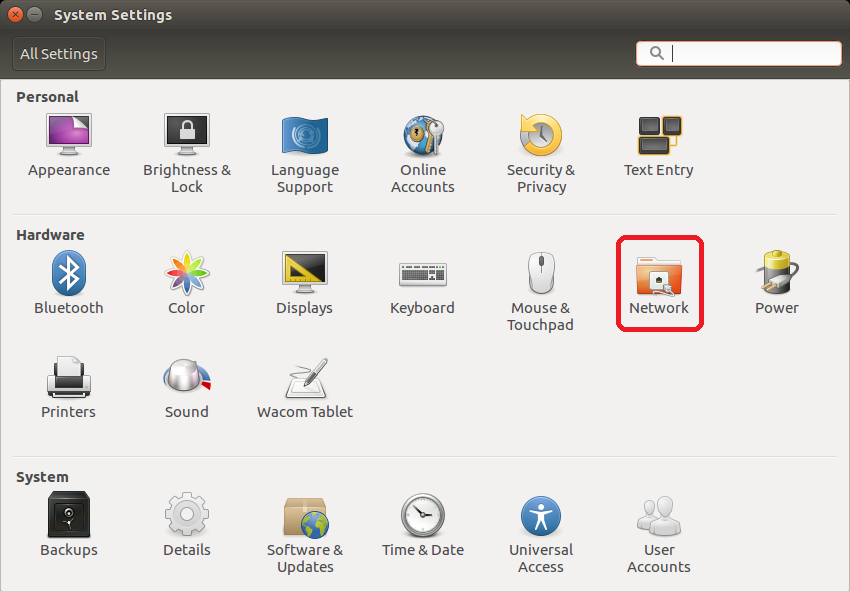
\includegraphics[width=0.5\textwidth,height=\textheight]{figures/geekbot/eth_config/system_settings.png}

\begin{enumerate}
\def\labelenumi{\arabic{enumi}.}
\setcounter{enumi}{1}
\tightlist
\item
  Select the wired network and in the lower-righthand side of the pane
  click 'Options'. Here we can change specific settings for how Ubuntu
  handles the Ethernet port of your computer.
\end{enumerate}

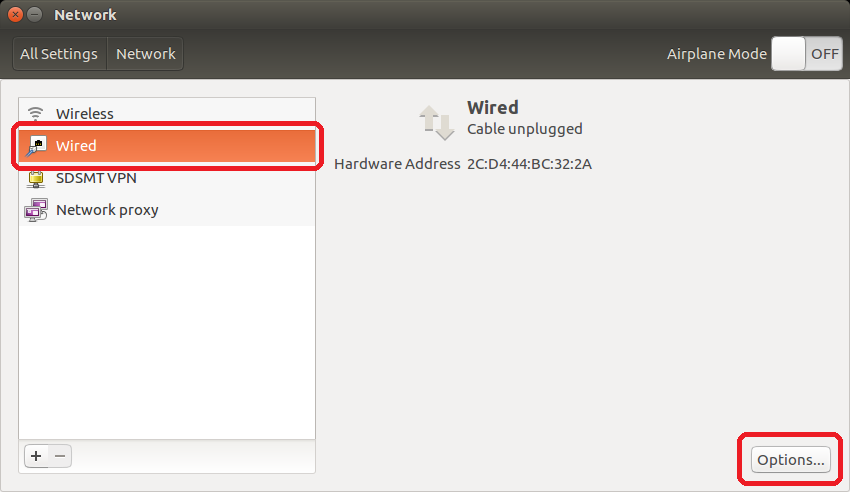
\includegraphics[width=0.5\textwidth,height=\textheight]{figures/geekbot/eth_config/network_wired.png}

\begin{enumerate}
\def\labelenumi{\arabic{enumi}.}
\setcounter{enumi}{2}
\tightlist
\item
  Click on the IPv6 tab. In the drop down, select 'Ignore'. We won't be
  using IPv6 to connect to the GeekBots.
\end{enumerate}

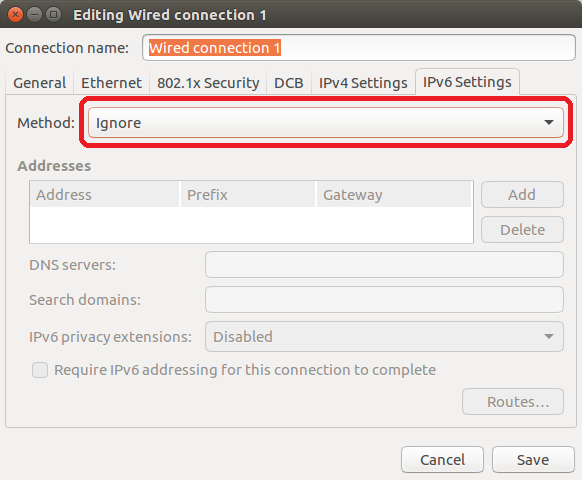
\includegraphics[width=0.5\textwidth,height=\textheight]{figures/geekbot/eth_config/ipv6_ignore.png}

\begin{enumerate}
\def\labelenumi{\arabic{enumi}.}
\setcounter{enumi}{3}
\tightlist
\item
  Now select the IPv4 tab and choose 'Share to other computers' from the
  dropdown menu. In the lower right hand corner click 'Save'.
\end{enumerate}

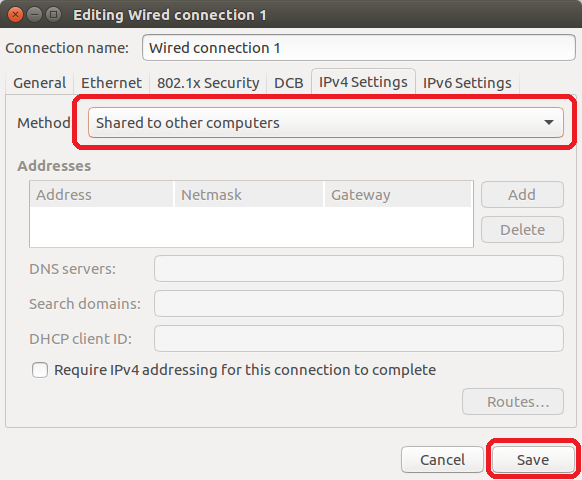
\includegraphics[width=0.5\textwidth,height=\textheight]{figures/geekbot/eth_config/ipv4_shared.png}

The Ethernet port on your computer is now set to automatically assign an
IP on 10.42.0.X spectrum to anything connected to it and requesting an
IP address. This is the default state of the GeekBot, so if the GeekBot
is connected to your computer then it will request and be assigned an IP
in the 10.42.0.X range.

\hypertarget{connecting-to-the-geekbot}{%
\subsubsection{Connecting to the
GeekBot}\label{connecting-to-the-geekbot}}

\begin{enumerate}
\def\labelenumi{\arabic{enumi}.}
\tightlist
\item
  Connect an Ethernet cable between your computer and the GeekBot's
  Odroid.
\item
  Power on the GeekBot by flipping the switch in the left-rear of the
  bot outwards. The Odroid and Arduino should start flashing lights.
\item
  Wait patiently for the Odroid to boot. This should take
  \textasciitilde30 seconds. When the Odroid has finished the booting
  process and has grabbed an IP from your computer, it will launch its
  ROS system and initiate communications with the onboard Arduino. If a
  successful connection is made \emph{you will hear two beeps from the
  robot}.
\item
  Navigate to the geekbot\_resources folder you cloned in the initial
  setup. Source the \texttt{geekbot\_connect.source} file. This will use
  \texttt{nmap} to scrape the 10.42.0.X subnet looking for your bot, set
  the necessary environment variables, and automatically load in ROS
  Kinetic to this specific terminal instance.
\item
  If you see a list of topics print out to your terminal you have
  successfully connected! \textbf{You will have to follow step \#4 for
  each terminal instance you would like to connect to the GeekBot.}
\end{enumerate}

\hypertarget{shutting-down-the-geekbot}{%
\subsubsection{Shutting down the
GeekBot}\label{shutting-down-the-geekbot}}

\begin{enumerate}
\def\labelenumi{\arabic{enumi}.}
\tightlist
\item
  Flip the power switch in the left-rear of the bot forward, into the
  robot. If the power is off no lights should be on.
\end{enumerate}

\hypertarget{charging-the-geekbot}{%
\subsubsection{Charging the GeekBot}\label{charging-the-geekbot}}

\begin{enumerate}
\def\labelenumi{\arabic{enumi}.}
\tightlist
\item
  Locate your GeekBot battery charger. This is a wall-wart supply that
  has a ribbed back section, a little LED in the bottom left corner, a
  yellow tip, and an 8.4v 2A output.
\item
  Plug the charger into an outlet.
\item
  Locate the battery charging port on the front of the robot. This
  should be zip-tied down to the lower platform and will run directly
  into the battery.
\item
  Plug in the charger to the charging port. The light on the charger
  should become red. When fully charged, the light will turn green.
  These batteries have automatic over-voltage protection, so the charger
  can be left on the battery indefinitely.
\end{enumerate}

\hypertarget{running-the-geekbot-from-external-power}{%
\subsubsection{Running the GeekBot from external
power}\label{running-the-geekbot-from-external-power}}

\begin{enumerate}
\def\labelenumi{\arabic{enumi}.}
\tightlist
\item
  Make sure the GeekBot is powered off.
\item
  Disconnect the battery from the 2x5.5mm splitter zip-tied to the
  rear-right vertical support on the bot. Connect a power supply from
  7v-8.5v, or the battery charger provided with the robot.
\item
  If the charger for the battery is used be aware: this supply does not
  provide enough power to run both motors as well as intense computation
  on the Odroid. If your robot is intermittently losing connection when
  operating the motors with this supply you are most likely browning out
  the Odroid.
\end{enumerate}

\hypertarget{using-the-geekbot}{%
\subsection{Using the GeekBot:}\label{using-the-geekbot}}

\hypertarget{ros-in-built-tools}{%
\subsubsection{ROS' in-built tools}\label{ros-in-built-tools}}

When debugging ROS-based systems it can be very handy to peek in on what
data is being published on what topics by what nodes. We can accomplish
this easily with ROS' in-built command line tools. In ROS1 these take
the form of \texttt{rosxxxx} where \texttt{xxxx} roughly describes the
useful area of ROS within which we want to operate. For example,
listening in on a topic and pushing its published info to the screen can
be accomplished by using the \texttt{rostopic} tool:

\begin{quote}
\texttt{rostopic\ echo\ /geekbot/ir\_cm}
\end{quote}

Running the above you should see something like this on your screen:

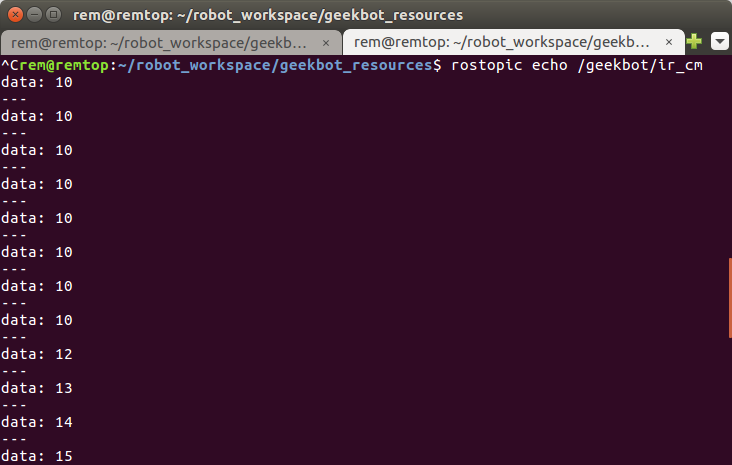
\includegraphics[width=0.7\textwidth,height=\textheight]{figures/geekbot/repo_usage/echo_ir.png}

The data presented is the Int32 payload published to the topic
\texttt{/geekbot/ir\_cm}. Maybe we want to see how fast new information
to this topic is being published. To do so we use the \texttt{rostopic}
tool yet again:

\begin{quote}
\texttt{rostopic\ hz\ /geekbot/ir\_cm}
\end{quote}

You should now see the average publishing rate, calculated standard
deviation for the publishing gap times, and also the number of samples
the stats were generated from:

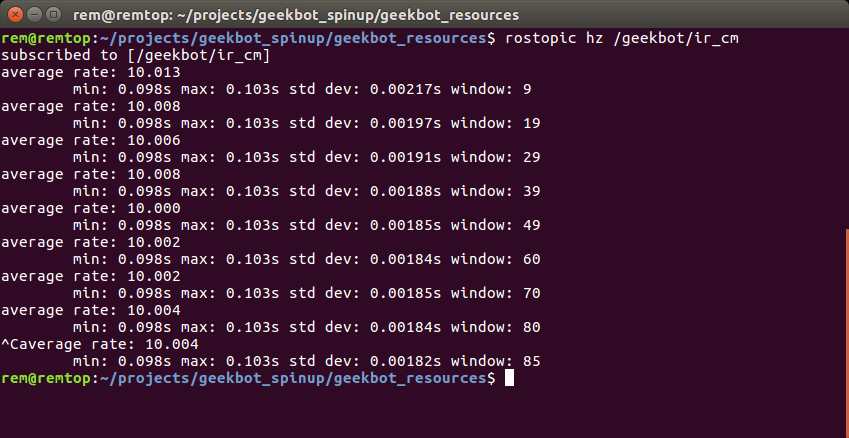
\includegraphics[width=0.7\textwidth,height=\textheight]{figures/geekbot/repo_usage/hz_ir.png}

It looks like the IR data is coming in at exactly 10hz as expected.
Neat!

We can also publish to a topic using the command line, using the
\texttt{rostopic\ pub} command. Tab-complete is very handy here. If
\texttt{rostopic} can't automatically find a list of topics you can
manually list registered topics with \texttt{rostopic\ list} and find
the topic type with \texttt{rostopic\ type}. Usually slapping the tab
key will give you options or autofill. To publish a single message
setting the left wheel speed of our GeekBot to 50\% power, the command
would look like the following:

\begin{quote}
\texttt{rostopic\ pub\ -\/-once\ /geekbot/left\_wheel\ std\_msgs/Int32\ "data:\ 50"}
\end{quote}

This will publish to the topic one message with the payload as
described:

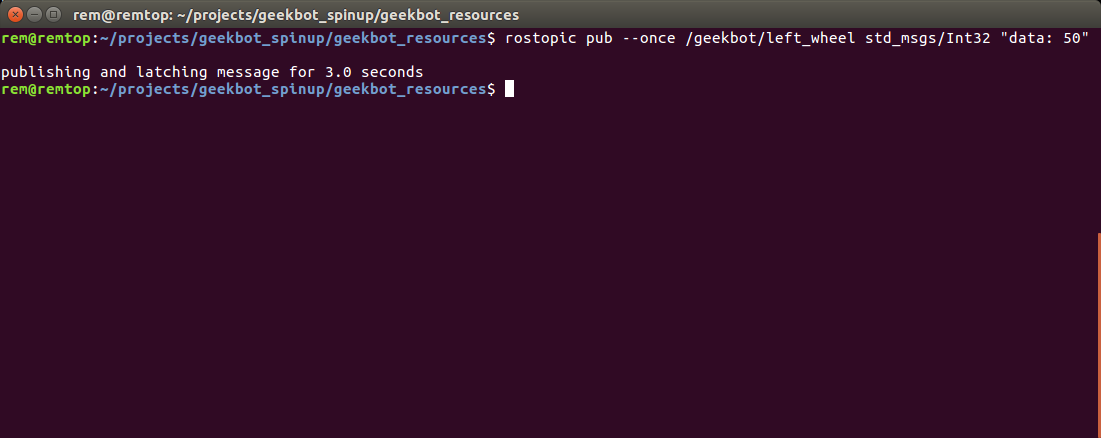
\includegraphics[width=0.7\textwidth,height=\textheight]{figures/geekbot/repo_usage/drive_left.png}

Your GeekBot's left wheel should start spinning! Remember: since we only
published a single message that wheel will keep spinning until we set
the speed back to zero. For more complex messages, let tab-complete do
the hard YAML work for you, then plug in your values. The following
example call uses a six-field Twist message, which the Geekbots do not
use:

\begin{verbatim}
rostopic pub --once /takes_a/twist_msg geometry_msgs/Twist \
"linear:
   x: 1.3
   y: 0.0
   z: 0.0
angular:
   x: 0.0
   y: 3.7
   z: 0.0"
\end{verbatim}

We can also list the nodes currently running and tracked by the
GeekBot's \texttt{roscore}:

\begin{quote}
\texttt{rosnode\ list}
\end{quote}

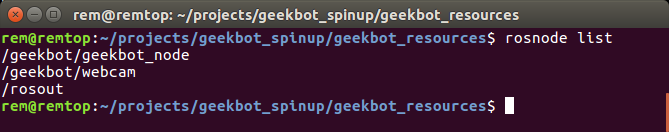
\includegraphics[width=0.7\textwidth,height=\textheight]{figures/geekbot/repo_usage/rosnode_list.png}

This shows the three nodes running in the GeekBot's namespace:
geekbot\_node, webcam, and rosout. Wouldn't it be neat if we could
easily visualize what nodes were running and over what topics they were
communicating? ROS has a tool for this! In one terminal echo the output
of the topic \texttt{/geekbot/ir\_cm}:

\begin{quote}
\texttt{rostopic\ echo\ /geekbot/ir\_cm}
\end{quote}

In another, use \texttt{rosrun} to run the ROS tool \texttt{rqt\_graph}:

\begin{quote}
\texttt{rosrun\ rqt\_graph\ rqt\_graph}
\end{quote}

This will run the pre-installed 'node' \texttt{rqt\_graph} in the
package \texttt{rqt\_graph} and generate a topic/node map! You should
see something like this:

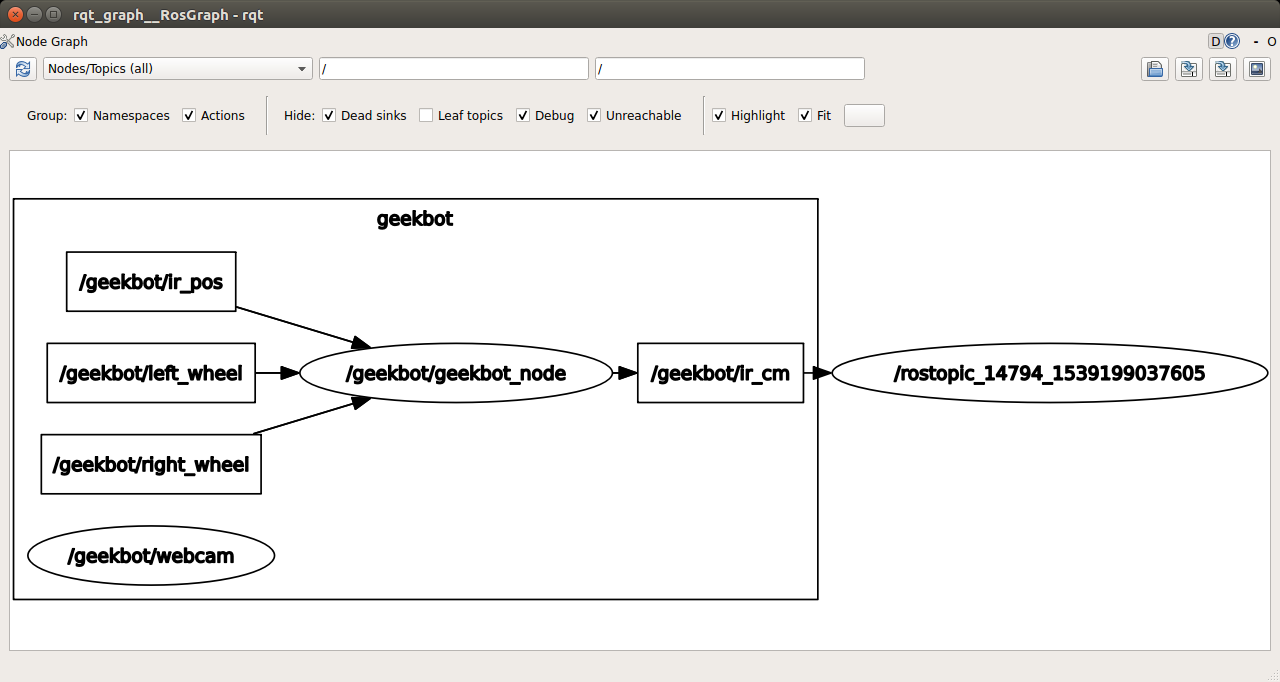
\includegraphics[width=0.7\textwidth,height=\textheight]{figures/geekbot/repo_usage/rqt_graph.png}

You can see the \texttt{/geekbot} namespace contains two nodes and
several topics. The node that exists outside of the \texttt{/geekbot}
namespace is the node created by \texttt{rostopic\ echo}.
\texttt{geekbot\_node} publishes messages to the
\texttt{/geekbot/ir\_cm} topic, and the \texttt{/rostopic\_.........}
node is subscribed to this topic. The arrows indicate message flow.
\texttt{rqt\_graph} is a very handy tool for debugging and
conceptualizing ROS systems. For large systems it is a necessity!

\hypertarget{sensor-driven-motion}{%
\subsubsection{Sensor-driven motion}\label{sensor-driven-motion}}

Inside the
\texttt{geekbot\_resources/examples/python\_examples/basic\_ir}
directory you should see a file named \texttt{ir\_drive.py}. This script
contains:

\begin{Shaded}
\begin{Highlighting}[]
\CommentTok{\#!/usr/bin/env python}
\ImportTok{import}\NormalTok{ rospy}
\ImportTok{from}\NormalTok{ std\_msgs.msg }\ImportTok{import}\NormalTok{ Int32}

\NormalTok{left\_pub }\OperatorTok{=}\NormalTok{ rospy.Publisher(}\StringTok{\textquotesingle{}/geekbot/left\_wheel\textquotesingle{}}\NormalTok{, Int32, queue\_size}\OperatorTok{=}\DecValTok{10}\NormalTok{)}
\NormalTok{right\_pub }\OperatorTok{=}\NormalTok{ rospy.Publisher(}\StringTok{\textquotesingle{}/geekbot/right\_wheel\textquotesingle{}}\NormalTok{, Int32, queue\_size}\OperatorTok{=}\DecValTok{10}\NormalTok{)}

\KeywordTok{def}\NormalTok{ callback(data):}
\NormalTok{    rospy.loginfo(rospy.get\_caller\_id() }\OperatorTok{+} \StringTok{" IR: }\SpecialCharTok{\%s}\StringTok{"}\NormalTok{, data.data)}
    \ControlFlowTok{if}\NormalTok{ data.data }\OperatorTok{\textless{}} \DecValTok{15}\NormalTok{:}
        \BuiltInTok{print}\NormalTok{(}\StringTok{"Driving forward."}\NormalTok{)}
\NormalTok{        msg }\OperatorTok{=}\NormalTok{ Int32()}
\NormalTok{        msg.data }\OperatorTok{=} \DecValTok{50}
\NormalTok{        left\_pub.publish(msg)}
\NormalTok{        right\_pub.publish(msg)}
    \ControlFlowTok{else}\NormalTok{: }
        \BuiltInTok{print}\NormalTok{(}\StringTok{"Too far! Stop!"}\NormalTok{)}
\NormalTok{        msg }\OperatorTok{=}\NormalTok{ Int32()}
\NormalTok{        msg.data }\OperatorTok{=} \DecValTok{0}
\NormalTok{        left\_pub.publish(msg)}
\NormalTok{        right\_pub.publish(msg)}

\KeywordTok{def}\NormalTok{ listener():}
\NormalTok{    rospy.init\_node(}\StringTok{\textquotesingle{}drive\_node\textquotesingle{}}\NormalTok{, anonymous}\OperatorTok{=}\VariableTok{True}\NormalTok{)}
\NormalTok{    rospy.Subscriber(}\StringTok{"/geekbot/ir\_cm"}\NormalTok{, Int32, callback)}
\NormalTok{    rospy.spin()}

\ControlFlowTok{if} \VariableTok{\_\_name\_\_} \OperatorTok{==} \StringTok{\textquotesingle{}\_\_main\_\_\textquotesingle{}}\NormalTok{:}
\NormalTok{    listener()}
\end{Highlighting}
\end{Shaded}

All this code does is instantiate a ROS node that subscribes to the
\texttt{/geekbot/ir\_cm} topic and publishes wheel speeds based on the
distance to the nearest object as determined by the front-mounted IR
sensor. When run on your computer the GeekBot should sit patiently until
you hold your hand within 15cm of the IR sensor. Then, it will drive
forward! This is reversed logic from what we often want (drive until
something gets in the way), but this way the GeekBot won't drive off
your desk the moment the code starts executing. Consider this a friendly
reminder to always prop up your robots so the wheels are off the ground
when testing motion code.

Plotting the ROS graph with \texttt{rqt\_graph} shows us that, indeed,
the \texttt{ir\_drive} node is indeed subbed to one topic and publishing
to both wheels:

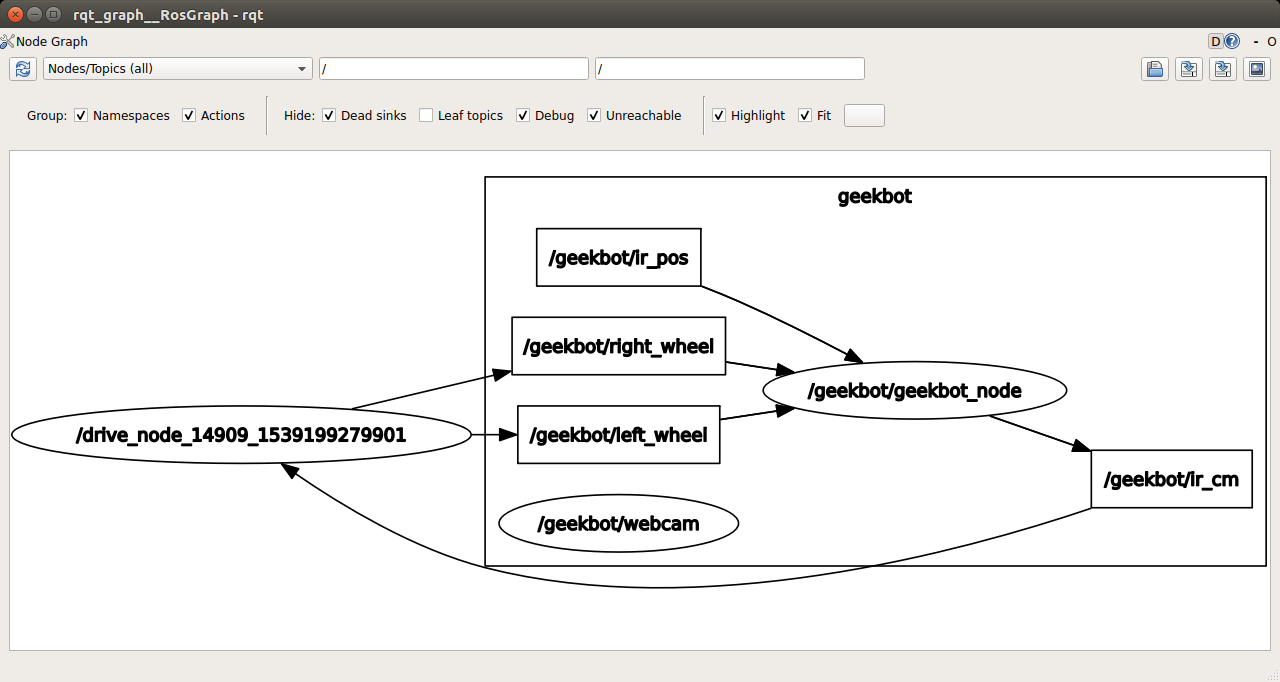
\includegraphics{figures/geekbot/repo_usage/drive_node.png}

\hypertarget{basic-computer-vision}{%
\subsubsection{Basic computer vision}\label{basic-computer-vision}}

Inside the
\texttt{geekbot\_resources/examples/python\_examples/basic\_cv}
directory you should see a file named \texttt{hsv\_detect.py}. This
script contains a bit too much code to prudently list here, so please
open it in your editor of choice and read along. An online copy can be
found on
\href{https://github.com/sdsmt-robotics/geekbot_resources/blob/master/examples/python_examples/basic_cv/hsv_detect.py}{this}
repo page. \textbf{BE WARNED} There's a bug in Python2.7's
muli-threading library that is known and will not be fixed. More info in
the code itself. \emph{Expect crashes.}

This code demonstrates 'elementary' computer vision capability using
OpenCV to process images communicated over a ROS-based image stream. To
use it you will need to install the \texttt{cv\_bridge} package to
convert between ROS CompressedImage messages and an image format OpenCV
understands:

\begin{quote}
\texttt{sudo\ apt\ install\ ros-kinetic-cv-bridge}
\end{quote}

With the bridge installed we can run the script. Upon running you should
see two windows: in one a camera stream from the GeekBot, the other a
black image. Move the 'maximum' sliders around. You should see pieces of
the camera feed start to come into frame and maybe a few rectangles
popping up. Set a high-color object in the camera's field of view and
adjust the sliders to home in on just this color. Blues and yellows work
well for this. With a bit of tinkering you should see something like
this:

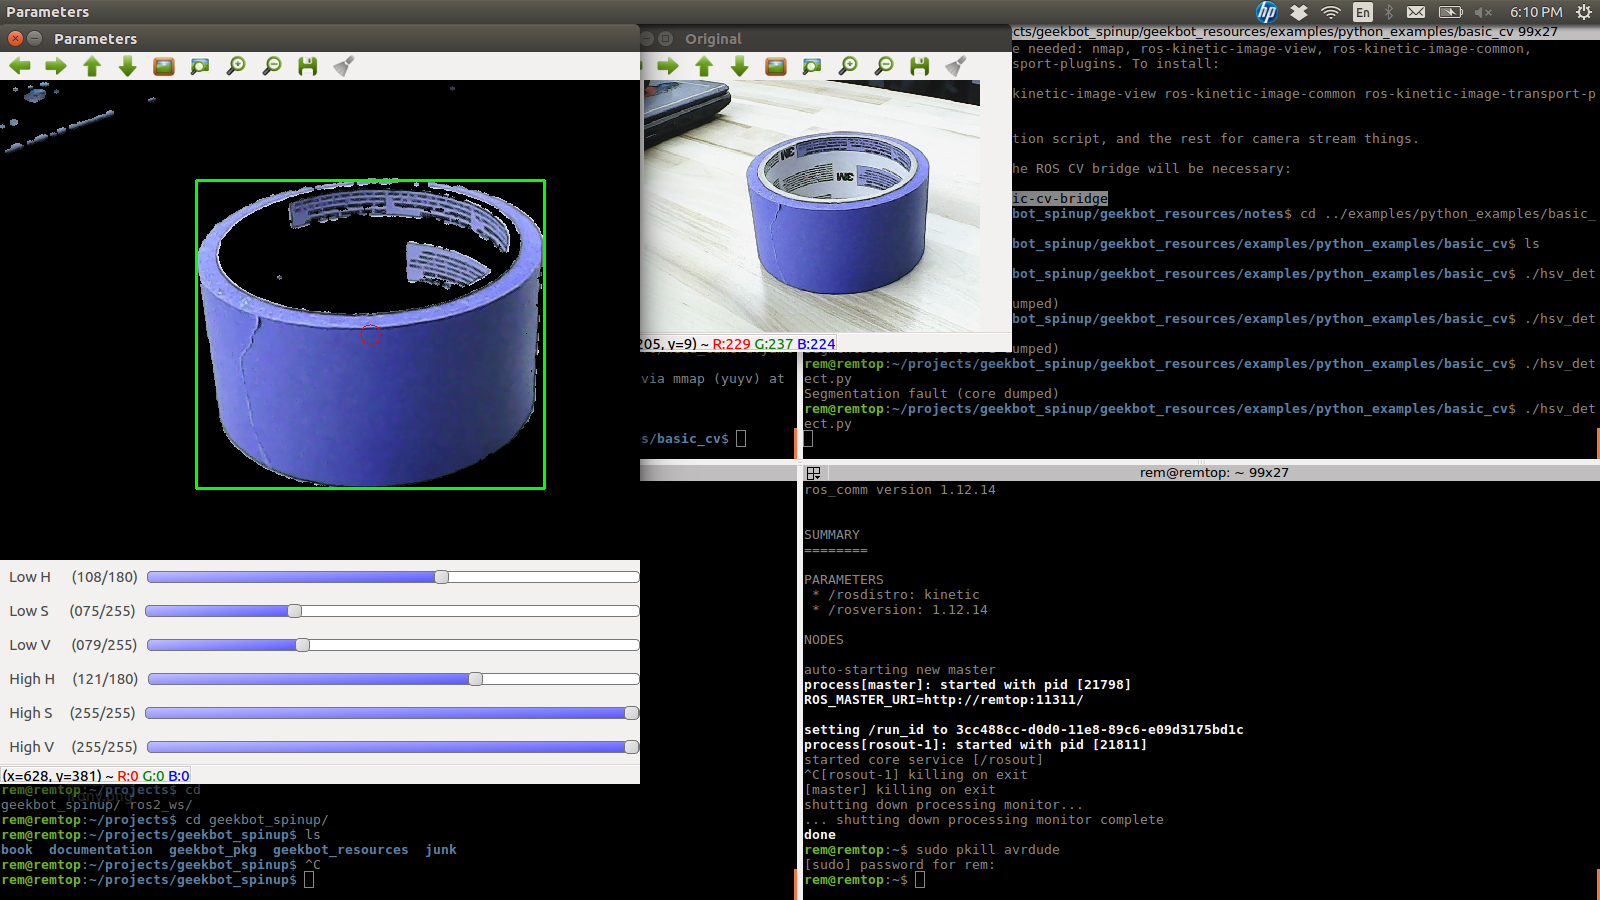
\includegraphics{figures/geekbot/repo_usage/cv_detect.png}

You will notice that the rectangle on screen is now bounding the object
with a red circle drawn in the center of the rectangle. Hooray: object
tracking by color extraction!

Here's a rough rundown of what's happening in the code, starting at
initial execution:

\begin{quote}
\begin{enumerate}
\def\labelenumi{\arabic{enumi}.}
\tightlist
\item
  Create an object\_tracker object, initialize the node and start
  processing
\item
  When an image is published to the
  \texttt{/geekbot/webcam/image\_raw/compressed} topic, convert it for
  OpenCV use
\item
  Make a copy of the original image and convert this copy to
  \href{https://en.wikipedia.org/wiki/HSL_and_HSV}{HSV} from RGB
\item
  Threshold the HSV copy by the min and max values determined from the
  sliders. This returns a binary mask
\item
  Denoise the mask with a series of dilations and erodes
\item
  Find all connected contours in the mask. These contours are individual
  blobs in the mask
\item
  Given a contour, generate a bounding rectangle for the contour. If the
  bounded area is too small, reject the rectangle
\item
  Given a list of all viable bounding rectangles, find the largest
\item
  Bitwise AND the adjusted mask with the original image. This will block
  anything not captured in the mask
\item
  Draw the largest rectangle (and its center) on on the now-reduced
  original image
\item
  Display all images to their respective windows
\end{enumerate}
\end{quote}

The code might look intimidating off the cuff but it really is this
straightforward. Conversion to the HSV colorspace is necessary to
produce a consistent color lock regardless of color brightness. A quick
online search will yield a variety of explanations that will be far more
useful than any discussion of HSV's merits for computer vision in this
text.

Notice that this code tracks the center of a bounding box. For the most
part this center will be near the centroid of a tracked object. Using
this information our GeekBot could be configured to automatically turn
itself when a tracked object gets too close to the edge of the frame.
The implementation of this (and other computer vision adventures) is
left to the reader.
